\subsection{Architectural design}
\subsubsection{Database}
The data layer interfaces itself only with the application layer, in particular with the subcomponent called "data manager". Besides the database engine, this layer is composed by a DBMS, which is in main part relational. The relational approach offers advantages ranging from the easy extensibility to independency from the physical organization, and in general the ACID properties of its transactions. For all these reasons fixed in front data and those that change less frequently are committed to the RDBMS, while for the others a NoSQL is provided. In fact thanks to its well-known scalability it fits better for data accumulated in large numbers every second, which is the case of all the data collected by the application through the wearable device.

The data layer has to store all the data shown in the following ER diagram, the sensible of which must be encrypted before being stored.

\begin{center}
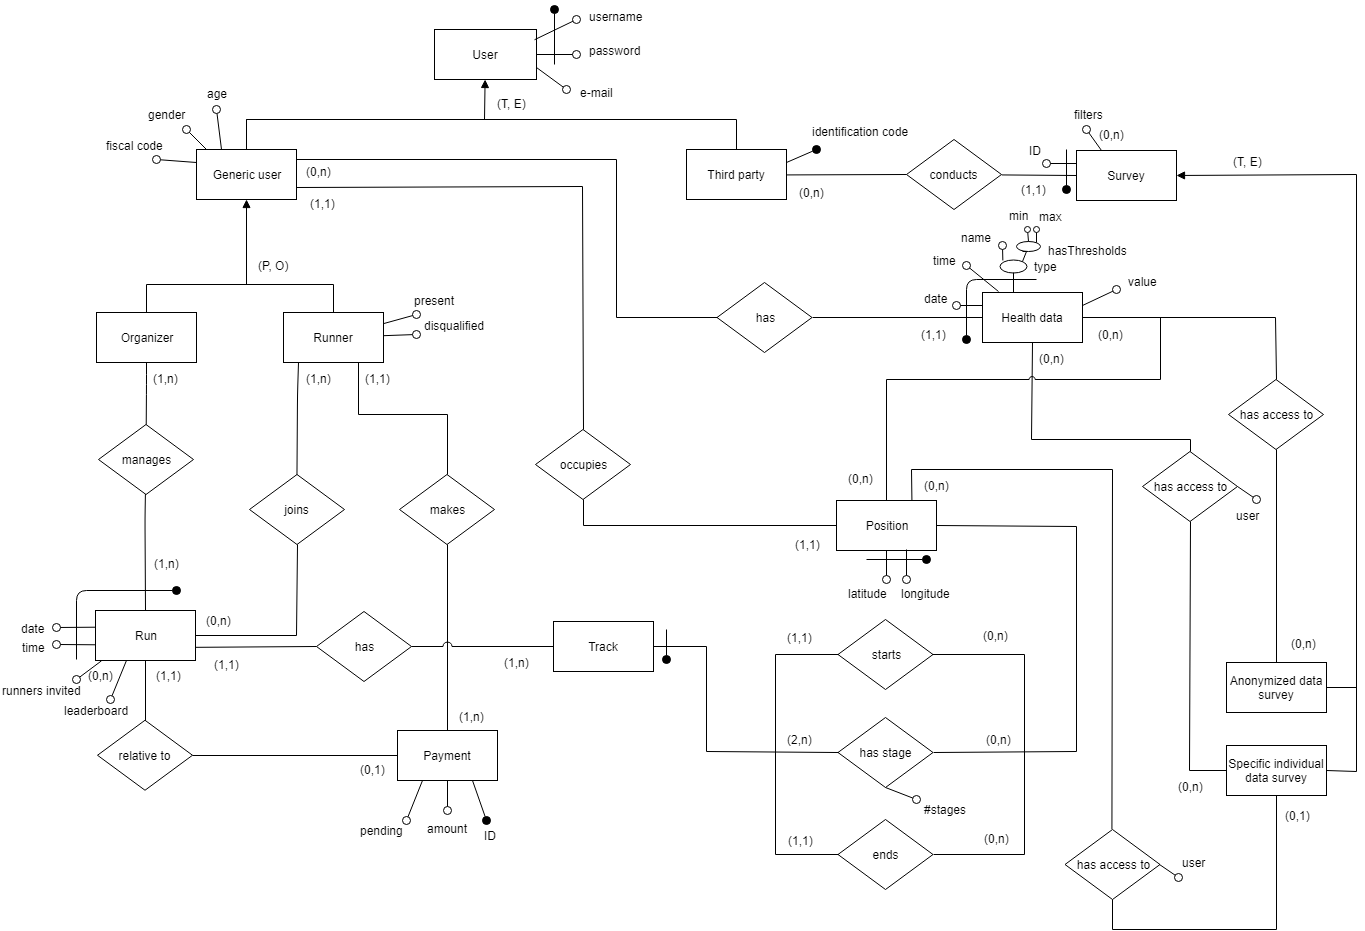
\includegraphics[scale=0.35]{sections/diagrams/ER.png}
\end{center}